% Milestone 4: Project Check-In. Build: tectonic m4.tex
\documentclass[10pt]{article}

\usepackage{fontspec}
\setmainfont{texgyrepagella}[Extension=.otf,UprightFont=*-regular,BoldFont=*-bold,ItalicFont=*-italic,BoldItalicFont=*-bolditalic]
\setsansfont{texgyreheros}[Extension=.otf,UprightFont=*-regular,BoldFont=*-bold,ItalicFont=*-italic,BoldItalicFont=*-bolditalic,Scale=0.96]
\setmonofont{texgyrecursor}[Extension=.otf,UprightFont=*-regular,BoldFont=*-bold,ItalicFont=*-italic,BoldItalicFont=*-bolditalic,Scale=0.88]

\usepackage[letterpaper,left=0.9in,right=0.9in,top=0.8in,bottom=0.8in]{geometry}
\usepackage{microtype}
\usepackage{xcolor}
\usepackage{booktabs,longtable,array}
\setlength{\LTpre}{0.2em}\setlength{\LTpost}{0.1em}
\usepackage{enumitem}
\usepackage{needspace}
\widowpenalty=10000 \clubpenalty=10000
\usepackage{tikz}
\usepackage{fancyhdr}
\usepackage[hidelinks]{hyperref}

\definecolor{tracerteal}{HTML}{2E6B66}
\definecolor{tealsoft}{HTML}{E2EDEB}
\definecolor{muted}{HTML}{5A6763}
\definecolor{hair}{HTML}{D9E0DD}
\definecolor{late}{HTML}{B0442F}
\definecolor{amber}{HTML}{A26A14}
\definecolor{okgreen}{HTML}{2F7A4F}

\setlength{\parindent}{0pt}
\setlength{\parskip}{0.45em}
\renewcommand{\arraystretch}{1.22}
\setlist{nosep,leftmargin=1.35em,itemsep=0.28em,topsep=0.25em}
\emergencystretch=2em

\pagestyle{fancy}
\fancyhf{}
\renewcommand{\headrulewidth}{0pt}
\lhead{\sffamily\scriptsize\color{muted}Tracer \textbullet\ Milestone 4: Project Check-In}
\rhead{\sffamily\scriptsize\color{muted}Escalante \textbullet\ Kocourek}
\cfoot{\sffamily\scriptsize\color{muted}\thepage}

% One numbered question: rule, number, question text, then the answer follows.
\newcommand{\qa}[2]{%
  \par\Needspace{6\baselineskip}\addvspace{0.75em}%
  {\color{hair}\rule{\textwidth}{0.5pt}}\par\nopagebreak\vspace{0.15em}%
  \noindent\hangindent=1.7em\hangafter=1
  {\sffamily\bfseries\color{tracerteal}\makebox[1.7em][l]{#1}\color{black}#2}\par\nopagebreak\vspace{0.1em}}

\newcommand{\status}[2]{\leavevmode{\sffamily\bfseries\footnotesize\color{#1}#2}}
\newcolumntype{L}[1]{>{\raggedright\arraybackslash}p{#1\textwidth}}
\newcommand{\repo}{\href{https://github.com/scalinity/Tracer}{\nolinkurl{github.com/scalinity/Tracer}}}

\hypersetup{pdftitle={Milestone 4: Project Check-In (Tracer)},pdfauthor={Karissa Kocourek and Daniel Escalante},pdfsubject={CAI 5724 AI in Health Design Studio I}}
\begin{document}

% ---------------------------------------------------------------- title block
{\raggedright
{\sffamily\bfseries\fontsize{21}{24}\selectfont Milestone 4: Project Check-In}\par\vspace{0.1em}
{\itshape\large Tracer: predictive specimen tracking for the clinical microbiology laboratory}\par\vspace{0.35em}
{\sffamily\footnotesize\color{muted}CAI 5724 AI in Health Design Studio I \textbullet\ University of Florida \textbullet\
Team: Karissa Kocourek and Daniel Escalante \textbullet\ October 28, 2026}\par}
\vspace{0.2em}{\color{tracerteal}\rule{\textwidth}{1.4pt}}

% ------------------------------------------------------------------------- 1
\qa{1.}{What is your in-class presentation date?}
Wednesday, November 18, 2026. The interactive demo has to be functionally complete by then; it
is not required to be camera-ready until the December 2 deadline.

% ------------------------------------------------------------------------- 2
\qa{2.}{How confident are you that your project will be completed on time?}
\textbf{Moderately confident: 3 out of 5 today.} The design is finished, and our decision to generate the
dataset with the Claude API removes the largest build risk, a hand-built discrete-event simulator. Confidence
is not higher because no pipeline code exists yet and the sourced policy table is still outstanding, which
leaves 21 days to build, test and rehearse a working demo.

We expect to reach 4 out of 5 if two things hold on November 3: a validated pilot dataset exists, and Karissa's
first-pass policy table is in. If either slips, we cut in a fixed order: the gradient-boosted challenger model,
then the robustness checks, then the depth of the location-estimate evaluation. We keep the working core, which is
the risk model, the live board and the specimen timeline.

% ------------------------------------------------------------------------- 3
\qa{3.}{Overall, where does your AI system stand today? What is working? What isn't?}
The design is complete and the core mathematics runs, but nothing that depends on data is built yet.
No model has been fitted or evaluated, so we have no performance numbers.

\begin{longtable}{@{}L{0.27}L{0.17}L{0.50}@{}}
\toprule
\sffamily\small Component & \sffamily\small Status today & \sffamily\small Evidence \\
\midrule
\endhead
Problem framing, architecture, data model & \status{okgreen}{Done} &
  Milestones 1--3; \texttt{docs/architecture.md}; public repository \repo. \\
Case that public data cannot be used & \status{okgreen}{Done} &
  MIMIC-IV Demo check: 1,336 microbiology specimens stamped only at collection and at final result (median 80.1
  hours apart), with no receipt, transport or setup events. \\
Risk model (specimen status and arrival forecast) & \status{amber}{Scripted example only} &
  Closed-form mixture-survival model runs in our interactive system map with hand-set parameters. Nothing is
  fitted from data. \\
Location estimate & \status{amber}{Scripted example only} &
  Hidden semi-Markov forward filter over four transit states runs in the same map, with the same caveat. \\
Synthetic dataset & \status{amber}{Decided, not generated} &
  Claude API generator designed (Question 6); pilot run not started. \\
Specimen policy table (windows and citations) & \status{late}{Outstanding} &
  Not yet in the shared project folder. The windows in use are labeled as assumptions. \\
Search brief (LLM) & \status{late}{Not started} & Design only. \\
Pipeline, evaluation, live board & \status{late}{Not started} & The \texttt{src/} folders are empty. \\
\bottomrule
\end{longtable}

% ------------------------------------------------------------------------- 4
\qa{4.}{Describe any major challenges your team has faced.}
\begin{itemize}
\item \textbf{No public dataset covers the interval we monitor.} In the MIMIC-IV Demo, a specimen is stamped at
  collection and again when the final result is documented, and never in between. We tested using it to
  calibrate a simulator and rejected that: it is critical-care data (all 100 patients had an ICU stay, 38.3\%
  of specimens are blood cultures, which we exclude), and more rows from the same hospital would not change the
  population. We therefore chose to generate our own synthetic dataset. The cost is that every timing
  parameter is an assumption, so we label each one and stress-test it.
\item \textbf{The label depends on a clinical judgment.} A specimen is late only relative to a stability window
  and the event that stops the clock. Only Karissa can supply and cite those, so her policy table gates the
  target variable. The clock rule lives in configuration, so a change costs a re-run, not a rewrite.
\item \textbf{A model can only explain what its state space contains.} Our first location model blamed silence on
  ``lost'' (0.64 lost against 0.35 at the tube station) until we added an explicit ``stalled at station''
  state, which moved the same silence to 0.68 at the station and 0.31 lost.
\item \textbf{Schedule.} Our time so far went to framing, architecture and the data feasibility check rather than
  code. Engineering is one person's serial path (data, fit, models, demo), so each late stage delays the next.
\end{itemize}

% ------------------------------------------------------------------------- 5
\qa{5.}{Compare your current progress with the development timeline you proposed in the last milestone.}
Milestone 3 set five stages. Documentation and design are done. Engineering is about one to two weeks behind.

\begin{longtable}{@{}L{0.31}L{0.09}L{0.54}@{}}
\toprule
\sffamily\small Milestone 3 stage & \sffamily\small Target & \sffamily\small Where it stands on October 28 \\
\midrule
\endhead
1. Specimen policy and workflow specification & Oct 16 &
  \status{late}{Late.} Workflow map and failure modes are written. The sourced stability table is not delivered. \\
2. Simulated specimen dataset & Oct 23 &
  \status{late}{Late.} The approach changed to Claude API generation; generator and pilot not yet built. \\
3. Status and arrival forecast, minimum viable prototype & Oct 30 &
  \status{late}{Will be missed.} The model exists as running JavaScript with assumed parameters. The version fitted
  from data is not started. \\
4. Location estimate and search brief & Nov 13 &
  \status{amber}{At risk.} The location filter exists as running JavaScript on a scripted example. The search brief
  is not started. \\
5. Interactive demo tutorial & Dec 2 &
  \status{amber}{Seed only.} Our system map (\texttt{visuals/architecture.html}) is the starting point. A working
  version is now needed by Nov 18. \\
\bottomrule
\end{longtable}

% ------------------------------------------------------------------------- 6
\qa{6.}{Describe any changes to your Development Roadmap from the previous milestone.}
Unchanged are the four modules, the Nov 13 target for location and search brief, and the Dec 2 and Dec 9 deadlines. The changes are listed first; the figure after them puts the Milestone 3 plan (grey) and the revised plan (green) on one axis.

\begin{itemize}
\item \textbf{Data source.} The simulated dataset becomes a synthetic dataset generated with the Claude API.
  Seeded code draws each specimen's brief (type, tests, unit, hour, route, planted failure, timing targets);
  Claude writes the event trail and true location history for it; a validator checks timestamps, workflow order
  and the planted outcome; accepted output is frozen and committed. No public dataset has intermediate events,
  and building a discrete-event simulator would have cost weeks.
\item \textbf{Smaller, staged dataset.} About 12{,}000 specimens instead of 50{,}000, since the models fit a few
  parameters per specimen group and cost now scales with size. A 200-specimen pilot, reviewed by Karissa, comes first.
\item \textbf{Policy table split in two.} A provisional first pass (Nov 1) lets generation start; the cited
  version follows (Nov 8).
\item \textbf{Minimum viable prototype redefined} as the thinnest end-to-end path (data, fitted risk model,
  alerts, board and timeline), moved from Oct 30 to Nov 8, with the location estimate and search brief added by Nov 13.
\item \textbf{Demo pulled forward.} Functionally complete by Nov 16 for the Nov 18 presentation, camera-ready
  by Dec 2. It gains an audience activity and a 3D view of the specimen's journey, with a 2D fallback.
\end{itemize}

\begin{center}
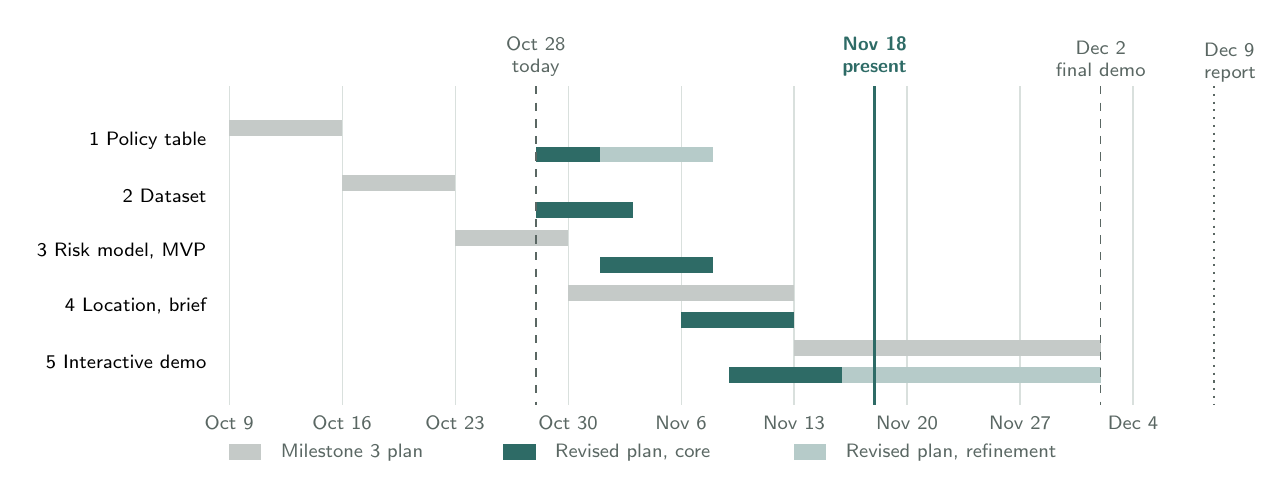
\begin{tikzpicture}[x=0.205cm,y=1cm,font=\sffamily\scriptsize]
  \def\ytop{0.35}
  % week ticks (Fridays)
  \foreach \d/\l in {0/Oct 9,7/Oct 16,14/Oct 23,21/Oct 30,28/Nov 6,35/Nov 13,42/Nov 20,49/Nov 27,56/Dec 4}{
    \draw[hair] (\d,\ytop) -- (\d,-3.7);
    \node[color=muted,anchor=north] at (\d,-3.72) {\l};
  }
  % stage rows
  \foreach \i/\name/\a/\b/\ra/\rb/\rc in {
    1/{1  Policy table}/0/7/19/23/30,
    2/{2  Dataset}/7/14/19/25/25,
    3/{3  Risk model, MVP}/14/21/23/30/30,
    4/{4  Location, brief}/21/35/28/35/35,
    5/{5  Interactive demo}/35/54/31/38/54}{
    \pgfmathsetmacro{\y}{-0.7*\i+0.35}
    \node[anchor=east,color=black] at (-0.8,\y) {\name};
    \fill[muted!35] (\a,\y+0.07) rectangle (\b,\y+0.27);
    \fill[tracerteal] (\ra,\y-0.27) rectangle (\rb,\y-0.07);
    \ifnum\rc>\rb
      \fill[tracerteal!35] (\rb,\y-0.27) rectangle (\rc,\y-0.07);
    \fi
  }
  % markers
  \draw[muted,dashed,thick] (19,\ytop) -- (19,-3.7);
  \node[color=muted,anchor=south,align=center] at (19,\ytop) {Oct 28\\today};
  \draw[tracerteal,very thick] (40,\ytop) -- (40,-3.7);
  \node[color=tracerteal,anchor=south,align=center,font=\sffamily\bfseries\scriptsize] at (40,\ytop) {Nov 18\\present};
  \draw[muted,dashed] (54,\ytop) -- (54,-3.7);
  \node[color=muted,anchor=south,align=center] at (54,\ytop) {Dec 2\\final demo};
  \draw[muted,dotted,thick] (61,\ytop) -- (61,-3.7);
  \node[color=muted,anchor=south west,align=left,inner sep=1pt] at (60.2,\ytop) {Dec 9\\report};
  % legend
  \fill[muted!35] (0,-4.4) rectangle (2,-4.2);
  \node[anchor=west,color=muted] at (2.6,-4.3) {Milestone 3 plan};
  \fill[tracerteal] (17,-4.4) rectangle (19,-4.2);
  \node[anchor=west,color=muted] at (19.6,-4.3) {Revised plan, core};
  \fill[tracerteal!35] (35,-4.4) rectangle (37,-4.2);
  \node[anchor=west,color=muted] at (37.6,-4.3) {Revised plan, refinement};
\end{tikzpicture}
\end{center}

% ------------------------------------------------------------------------- 7
\qa{7.}{List each dataset you are using, including links to any public datasets.}
\begin{longtable}{@{}L{0.21}L{0.73}@{}}
\toprule
\sffamily\small Dataset & \sffamily\small What it is and how we use it \\
\midrule
\endhead
\textbf{Tracer Synthetic Specimen Event Dataset} (our own; generated with the Claude API) &
  Event histories for five specimen types (urine, body fluid, bronchoalveolar lavage, culture swab, tissue), each with its
  ordered tests. Each record has scan events from collection to plating, the true location over time (held out, used
  only for evaluation) and outcome labels, with injected failures: lost in tube storage, stalled on the counter,
  misrouted, never sent, and content failures rejected at accessioning. Planned size: a 200-specimen pilot, then about
  12{,}000 specimens in 30 seeded runs of 7 days. All timing parameters are assumed and labeled; no patient or
  institutional data is used. Search briefs for each alert are generated with Claude and stored with it. Used to
  fit and test the modules and to power the demo. No external link: the generator, prompts, validators and frozen dataset
  (with a manifest of model, prompts and seeds) will be published in \repo. \\
\addlinespace
\textbf{Specimen Stability Reference Table} &
  Stability window and transport condition for each specimen type and test, one row each, with a citation, compiled from the
  \href{https://www.idsociety.org/practice-guideline/laboratory-diagnosis-of-infectious-diseases/}{IDSA and ASM Guide to
  Utilization of the Microbiology Laboratory} and, for swabs, the
  \href{https://www.copanusa.com/wp-content/uploads/2024/03/HPC030R05_PI-ESWAB-USA-2023.03.pdf}{eSwab manufacturer
  instructions}. Sets the time remaining before recollection and parameterizes the generator. \\
\addlinespace
\textbf{MIMIC-IV Clinical Database Demo v2.2} (\href{https://physionet.org/content/mimic-iv-demo/2.2/}{PhysioNet}) &
  100 critical care patients, 1,336 microbiology specimens. Not used to train any module. It is evidence that existing
  hospital data does not capture the interval Tracer monitors. \\
\bottomrule
\end{longtable}

% ------------------------------------------------------------------------- 8
\qa{8.}{List the major steps remaining to complete your project.}
\begin{enumerate}[leftmargin=1.5em]
\item \textbf{Policy table} (Karissa). First pass for five specimen types with window, transport and where the
  clock stops by \textbf{Nov 1}; cited version, alert routing and tolerable alerts per shift by \textbf{Nov 8}.
\item \textbf{Dataset} (Daniel; Karissa reviews 20 timelines). Build the brief sampler, Claude prompt and validator;
  validated pilot by \textbf{Oct 31}; full dataset frozen by \textbf{Nov 3}.
\item \textbf{Models and evaluation} (Daniel). Fit the interval distributions, build the risk model, a simple
  time-threshold baseline and the evaluation (median warning time, alerts per shift, catch rate, calibration)
  on held-out runs by \textbf{Nov 8}.
\item \textbf{Alerts, board and timeline} (Daniel; Karissa reviews sampled alerts) by \textbf{Nov 10}.
\item \textbf{Location estimate and search brief} (Daniel; Karissa reviews 20 briefs for clinical accuracy)
  by \textbf{Nov 13}, with the Claude brief compared against a fixed-template brief.
\item \textbf{Interactive demo} (Daniel builds; Karissa writes the clinical background and workflow narrative).
  Export results, build the tutorial, audience activity and 3D view, deploy to GitHub Pages. Functionally complete
  \textbf{Nov 16}; rehearsal Nov 16 to 17.
\item \textbf{Present} on \textbf{Nov 18}.
\item \textbf{Finish} the camera-ready prototype and demo by \textbf{Dec 2} and the final report by \textbf{Dec 9},
  drafting report sections alongside the build.
\end{enumerate}

% ------------------------------------------------------------------------- 9
\qa{9.}{Describe your plan for the in-class interactive demo (platform, where it runs, how students access it).}
\textbf{Platform.} A static interactive web page (HTML, CSS and JavaScript, no server) in \repo, hosted on GitHub
Pages. The Python prototype runs offline to fit the models and export results; the page reads those results and
the fitted parameters and re-computes risk and alerts live in the browser, so the demo uses the real prototype
rather than a mock-up.

\textbf{Where it runs and how students reach it.} In each student's own browser, on a phone or laptop, from a public
link and QR code shown in class and posted on Canvas. No HiPerGator, no hosted server, no install, no login and no
API key. We chose this over Streamlit or Jupyter because a server is one more thing to fail when a whole class
connects at once. Search briefs are generated with Claude ahead of time and stored with the results, so the demo
makes no live API calls. The same files open from disk, and we will keep a recorded walkthrough as a backup.

\textbf{What students can do} (about 10 minutes): watch a live board rank simulated specimens by risk; scrub a
timeline to see risk, likely location and expected arrival change while a specimen is silent; move the alert
threshold and see warning time against alerts per shift for Tracer and the baseline; try to call a missing
specimen before Tracer does; and view the specimen's journey in 3D.

% ------------------------------------------------------------------------ 10
\qa{10.}{List any remaining uncertainties, questions, or unresolved challenges.}
\begin{itemize}
\item \textbf{Will generated data be realistic enough?} We do not yet know how often Claude's trails will pass
  the validator, or whether they will be too uniform or have too thin a tail of late specimens. The pilot
  answers this before we spend more. Results will show that the models recover what we encode, not real-world
  performance, which is why we plan sensitivity analysis and will say so in the report.
\item \textbf{Where the clock stops.} Our working rule is collection to plating, from Karissa's bench knowledge.
  It defines the target variable, so it must be confirmed in the cited policy table. A change means re-running
  every fit.
\item \textbf{Alert budget and routing.} Six alerts per shift is our assumption; the number a laboratory would
  tolerate, and who acts on each failure type, are still Karissa's to confirm.
\item \textbf{Scope and devices.} Four modules in about three weeks is tight (cut order in Question 2). The 3D view
  depends on browser graphics support, so the 2D demo is the fallback.
\item \textbf{API credits and cost.} Generation runs on promotional credits and should cost well under \$25; we
  will set a hard spending limit and confirm the credits do not expire before November 18.
\item \textbf{Questions for the instructor.} (a) Does a static GitHub Pages page count as a publicly accessible
  interactive web application? (b) How long is each presentation slot? (c) What level of provenance detail do you
  expect in the final report for AI-generated synthetic data (we will record model, prompts, seeds and validation)?
  (d) Do the weekly draft milestones (Results on Nov 4, Discussion on Nov 11) still apply?
\end{itemize}

\end{document}
